\begin{comment}
	\subsection{Análise de Performance de Sistema}
\end{comment}


\section{Metodologia da Pesquisa}

\subsection{\Design\ Referencial de \Software\ para Sistemas Embutidos Utilizando Grafo de Controle de Fluxo} \label{chap:design} \label{sec:GCF}

	Segundo \cite{Sass2010} é possível descrever um sistema quanto em \hardware\ ou em \software\ livre de uma especificação de forma. 
    Uma delas é o desenvolvimento de rápidos protótipos referenciado como \design\ de referência de \software.
	Sua vantagem mais notável é a generalização de uma especificação de projeto bastante completa, eliminando qualquer tipo de incertezas sobre o comportamento do sistema com o simples fato de analisar o \design\ referencial do \software.
	% além de outras como o fato de que sua especificação pode ser analisada por ferramentas computacionais, e gerando modelos aut.

	%Assumindo que o \design\ de referência de \textit{software} já exista,
	%Aqui será demonstrado matematicamente como computação está em \design\ referencial de \software\ para que depois, isso possa nos auxiliar na decisão do que deverá ser implementado em nível de \hs. 
    Como o sistema a ser particionado é dado em forma de grafo de tarefas/rotinas, utiliza-se da teoria de grafos \cite{Mann2007}, em especial o gráfico de controle de fluxo (GCF). 
    Ele é definido por $ G = (B, F) $ onde $ B $ são vértices que representam os blocos básicos e $ F $ são arestas que indicam a todas as possibilidades de caminhos entre os blocos. 
    %Um exemplo é exibido na Figura \ref{fig:blocos_basicos}. O primeiro grupo \A\ é um bloco não básico porque não é maximal, ou seja, a primeira instrução \texttt{store word with update} deveria estar incluída ao grupo. Grupo \B\ é um bloco básico e o grupo \C\ não é pois existe duas entradas para o bloco, sendo elas na instrução \texttt{store word} e também pelo \texttt{branching} direcionado para \texttt{L2}.

	%Fazendo uma relação entre código em alto nível até o grafo de controle de fluxo, a Figura \ref{fig:f3-6} \textit{a)} exibe os blocos básicos em um código sem funcionalidade útil. Na Figura \ref{fig:f3-6} \textit{b)} é exibido o código gerado por um compilador para \texttt{PowerPC}\footnote{Arquitetura que utiliza RISC como arquitetura do conjunto de instruções.} onde os blocos básicos são identificados e por fim o gráfico de controle de fluxo, representado pela Figura \ref{fig:f3-6} \textit{c)}. Deve-se atentar que, só é possível identificar blocos básicos em um arquivo em linguagem de programação \textit{C} desde que se saiba qual compilador foi utilizado para emitir o código \assembly.
	\begin{comment}
	\begin{figure}[h] \centering
		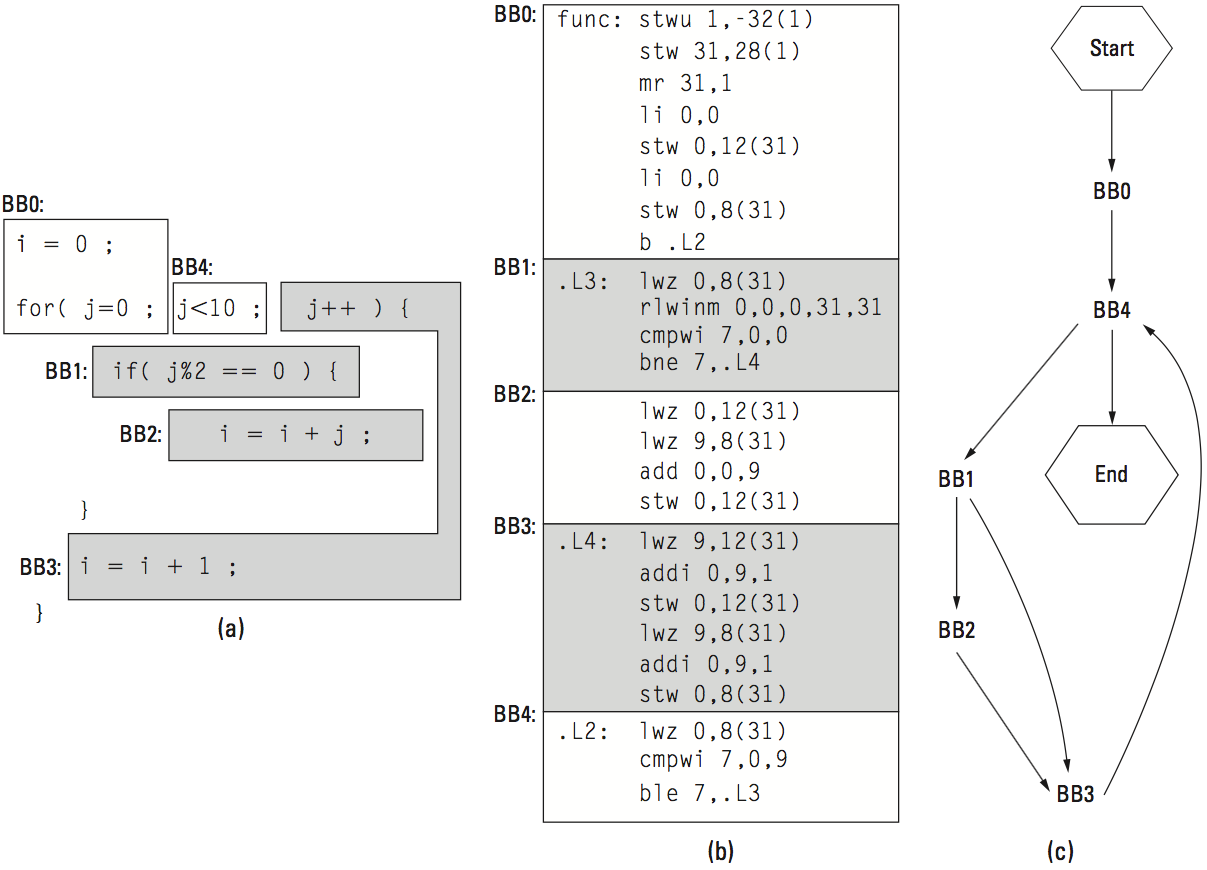
\includegraphics[width=0.9\textwidth]{img/f3-6.png}
		\caption{Identificação de blocos básicos e a representação de cada modelo de descrição de \software.}
		\label{fig:f3-6}
	\end{figure}
    \end{comment}

	Com a decomposição de um \design\ de referência de \software, gera-se dois componentes: uma porção a ser realizada em \hardware\ e outra executada em \software\ e essa decisão de divisão é chamada de problema de particionamento (descrito na Seção \ref{chap:desenvolvimento}).
    %Para sistemas baseados em Plataformas FPGA, particionamento é um sub-problema de um problema mais geral localizado no \codesign, onde refere-se ao \design\ cooperativo envolvendo \textit{stakeholders}, por exemplo.

	%Para continuar, deve-se definir alguns conceitos básicos, descritos na Seção \ref{sec:gc}.

\subsection{Grafo de Chamada} \label{sec:gc}
		\cite{Arato2003, Arato2005} \cite{Mann2007} \cite{Hassine2017} \todo{a} 
        
        Explicado como é modelado sub-rotina de um \design\ referencial de \software\ utilizando o grafo de controle de fluxo, agora será descrito o grafo de chamada (GC). Consiste num conjunto de GCFs, um por sub-rotinas, ou seja,

		\begin{equation}
			\mathcal{C} = {C_0, C_1, \dots C_{n-1}}
		\end{equation}

		%onde $ C_i = (V_i, E_i) $
		onde $ C_i = (B_i, F_i) $ representa o grafo de controle de fluxo de uma sub-rotina $ i $. Sendo assim, o grafo estático de chamada da aplicação é escrito por

		\begin{equation}
			\mathcal{A} = (\mathcal{C}, \mathcal{L}) \label{eq:a}
		\end{equation}

		onde $ \mathcal{A}$ representa uma aplicação específica e $ \mathcal{L} \subseteq \mathcal{C} \times \mathcal{C} $ é um subconjunto do plano cartesiano dos GCF. Duas sub-rotinas são relacionadas se podem ser determinadas, no tempo de compilação, que a sub-rotina $ i $ tem potencial de invocar a sub-rotina $ j $, ou seja, $ (C_i, C_j) \in \mathcal{L} $.

		É assumido que os blocos básicos de cada sub-rotina são disjuntos, ou seja, cada bloco básico em uma aplicação pertence a exatamente um GCF. Além do mais, é assumido que um nó raiz para o GC é implícito, ou seja, uma sub-rotina é designada a iniciar a execução.

		%Nem todos os executáveis podem ser expressados nesse modelo. Por exemplo, o manuseio de sinais e interrupções não são representadas e assim, não é possível determinar todos vértices $ F_i $ em uma dada sub-rotina $ C_i $ de um GCF antes da execução. 
        %Uma outra forma é com o paradigma de orientação à objeto. Ele depende do tempo de execução para conectar os métodos virtuais invocados e dessa forma, por \design, esse paradigma nos previne de saber todos os vértices antes da execução.
        %Para agora, será considerado que o modelo é suficiente para ser expressado em \design\ referencial de \software.

		Um equívoco comum é de que uma definição formal de particionamento só aplica à separação de aplicação componentes de \hs, ou seja, a partição contém exatamente dois conjuntos. 
        Todavia, para fazer o problema mais tratável, é comum agrupar primeiramente operandos em recursos, ou seja, uma partição com um grande número de subconjuntos, e então mapeia esses recursos tanto em \hardware\ quanto \software. 
        Assumindo que esses recursos atuam razoavelmente bem \textit{clustered}, então a decomposição de uma aplicação em componentes de \hs\ pode ser dirigida por comparações de ganho de performance desse recurso contra outro situado no outro conjunto. \todo{reler}

		Uma partição $ \mathcal{S} = \{S_0, S_1, \dots\}$ de um conjunto universal $ U $ é um conjunto de subconjuntos de $ U $ sendo que

		\begin{equation}
			\bigcup_{S \in \mathcal{S}} S = U \label{eq:part_form_1}
		\end{equation}
		\begin{equation}
			\forall S, S' \in \mathcal{S} | S \cap S' = \emptyset \label{eq:part_form_2}
		\end{equation}
        e assim
		\begin{equation}
			\forall S \in \mathcal{S} \cdot S \neq \emptyset \label{eq:part_form_3}
		\end{equation}

		A Equação \ref{eq:part_form_1} mostra que cada elemento de $ U $ é um membro de, pelo menos, um subconjunto $ S \in \mathcal{S} $. As Equação \ref{eq:part_form_2} e \ref{eq:part_form_3} dizem que os subconjuntos $ S \in \mathcal{S} $ são emparelhados disjuntos e não vazio. Em outras palavras, cada elemento do nosso universo $ U $ termina exatamente em um dos subconjuntos de $\mathcal{S}$ e nenhum dos subconjuntos são vazios.
		\begin{comment}
		Por exemplo, considerando as vogais da língua inglesa onde o universo $ U = \{a, e, i, o, u, y\} $. Assim, uma partição desse problema $ \mathcal{X}_a $ de $ U $ pode ser representado por


		\begin{equation}
			\mathcal{X}_a = \left\{\{a, e, i, o, u\}, \{y\}\right\} \label{eq:xa}
		\end{equation}

		e supondo que o conjunto pode ser representando por cada unidade, uma outra forma de representação pode ser


		\begin{eqnarray}
			\mathcal{X}_b &=& \left\{\{a\}, \{e\}, \{i\}, \{o\}, \{u\}, \{y\}\right\}
		\end{eqnarray}

		Sobre tais conceitos, a Partição \ref{eq:part_c} viola a Equação \ref{eq:part_form_1} e a Partição \ref{eq:part_d} viola as Equações \ref{eq:part_form_2} e \ref{eq:part_form_3}.

		\begin{eqnarray}
			\mathcal{X}_c &=& \left\{\{a\}, \{e\}, \{i\}, \{o\} \right\} \label{eq:part_c} \\
			\mathcal{X}_d &=& \left\{\{a, e, i\}, \{i, o, u, y\}, \{\}\right\} \label{eq:part_d}
		\end{eqnarray}

		A Figura \ref{fig:f4-2} ilustra o $ \mathcal{X}_a $ graficamente, segundo a Partição \ref{eq:xa}.

		\begin{figure}[h] \centering
			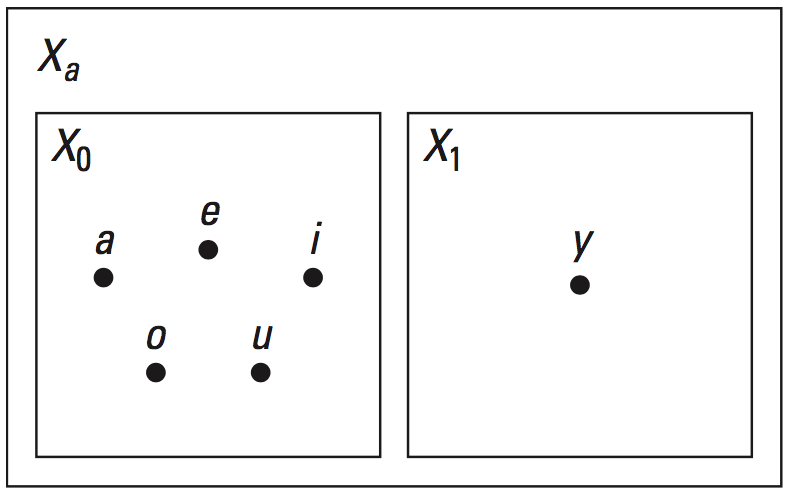
\includegraphics[width=0.5\textwidth]{img/f4-2.png}
			\caption{Figura representativa do mapeamento da aplicação.}
			\label{fig:f4-2}
		\end{figure}
		\end{comment}
		Aprendido os conceitos, é possível aplicar o formalismo à $ \mathcal{A} $. Se assumirmos que nosso universo é o conjunto de todos os blocos básicos $B$ de todas as sub-rotinas, então $U$ é as partições de sub-rotinas

		\begin{equation}
			U = \bigcup_{C \in \mathcal{C}} B(C) \label{eq:bigcup}
		\end{equation}

		 e chamaremos de partição natural da aplicação, onde
{ \footnotesize
		\begin{equation}
			\mathcal{S}  = \left \{
			\underbrace{\left \{ b_0, b_1, \dots, b_i \right \}}_{\text{sub-rotina }C_0},
			\underbrace{\left \{ b_i, b_{i+1}, \dots \right \}}_{\text{sub-rotina }C_1},\dots
			\underbrace{\left \{ b_j, b_{j+1}, \dots \right \}}_{\text{sub-rotina }C_{n-1}}
			\right \}
		\end{equation}
}

		Nossa tarefa será reorganizar a partição de blocos básicos e então mapear cada subconjunto de ambos os \hardwares\ e \software. Dessa forma, estamos livres para criar e remover subconjuntos não vazios, e mover blocos básicos ao redor até termos uma nova partição e assim termos um novo resultado $ \mathcal{A}’ = (\mathcal{C}’, \mathcal{L}’) $, inferido a partir da reorganização da partição $ \mathcal{X}’ $. O segundo passo é mapear cada subconjunto de $ \mathcal{X} $ para ambos \hs\ como é exibido abaixo

{ \tiny 
		\begin{equation}
			\mathcal{X}' = \left \{
			\underbrace{
            		\underbrace{
                    	\left \{ b_j, b_{j+1}, \cdots \right \}
                       }_{\text{sub-rotina }C_k}
                    \underbrace{
                    	\left \{ b_k, b_{k+1}, \cdots \right \}
                    }_{\text{sub-rotina }C_l}
                    \dots
                }_{\text{\software}}
                \
			\underbrace{
            		\underbrace{
            			\left \{ b_0, b_1, \cdots, b_i \right \}
                    }_{\text{sub-rotina }C_r}
                    \underbrace{
                        \left \{ b_i, b_{i+1}, \cdots \right \}
                    }_{\text{sub-rotina }C_s}
                    \dots
                }_{\text{\hardware}}
			\right \} \label{eq:part_final}
		\end{equation}
}


\subsection{Ganho de Performance} \label{sec:ganho_performance}
	Para explicar como performance pode ser utilizada para guiar o particionamento, será descrita uma métrica simples chamada taxa de execução.
	É parcialmente motivada pelo fato de que: \textit{a)} o ganho de performance é relativamente fácil de ser mensurado e \textit{b)} por causa de que, de todas as métricas comumente utilizadas, \speedup\ é frequentemente a mais importante. Diferente do mundo \software\ onde se tem análise de ordem de complexidade, em \hardware\ não possui-se um guia geral para comparação. O ganho de performance para aplicações em geral pode estar na acumulação de pequenos ganhos que deveriam ser perdido numa aplicação direta na teoria de complexidade.

	% tempo software
	Assim, será usado a informação de \profile\ (Seção \ref{sec:profile}) para coletar o tempo total de execução, bem com uma fração do tempo gasto em cada sub-rotina.
    O produto disso é a aproximação entre o tempo necessário para executar uma porção de aplicação em \software\ e usar isso como o tempo que se espera que tomará em futuras execuções. 
    Será utilizado $ s(i) $ para representar o tempo de execução esperado para uma invocação de uma sub-rotina $ i $, ou seja, bloco básico. 
    É considerado uma aproximação pois é dependente dos conjuntos de dados de entrada para muitas aplicações além da existência de erros que podem impactar a performance.

	% tempo hardware
	Precisa-se também aproximar o tempo que uma implementação equivalente em \hardware\ que iria tomar. 
    No caso dos blocos básicos implementados, isso é frequentemente mais preciso. 
    Como não possui-se um controle de fluxo, uma ferramenta auxiliar à síntese pode dar uma aproximação de acurácia de propagação de tempo.
    %Ou, se o recurso é \textit{pipelined}, o número de estágios é mais precisamente conhecido. Caso o recurso inclua controle de fluxo mas não contenha nenhum \textit{loop}, pode-se considerar o caminho mais longo como uma estimativa conservativa.

    Recursos com um número variável de iterações através de um \textit{loop} apresentam o maior obstáculo para encontrar um tempo de \hardware\ aproximado. 
    Nesse caso, implementação e \textit{profiling} com recurso em \hardware\ pode ser a única solução. 
    Independente, assume-se que uma aproximação apropriada $ h(i) $ para o existente tempo de execução em \hardware.

	% tempo mudanca de estado, configuracao, latencia
	Por fim, a interfaceação entre \hs\ requer tempo e este custo também precisa ser contabilizado. Pode-se aproximar deste custo pela aproximação do montante total do estado que necessita ser transferido ou o custo de configuração e latência. Em ambos os caso, são representados por $ m(i) $ para recursos $ i \in \mathcal{H} $, sendo $\mathcal{H}$ o conjunto de recursos do \hardware.

	% y é speedup
	%Taxa de execução é a velocidade na qual um sistema computacional completa uma aplicação, e em um sistema de plataforma FPGA olhamos para o \hardware\ para melhorar sua taxa de execução.
    O ganho, ao comparar uma solução \hs\ contra uma solução puramente \software, é tipicamente mensurado como \speedup. Utilizamos $ \gamma $ para sua representação e isso nos permitirá comparar recursos diferentes contra outros para determinar melhores particionamentos.
    Dessa forma, qualquer subconjunto de blocos básicos que não produzem um ganho de performance, podem ser excluídos de consideração. Em outras palavras, somente subconjuntos de blocos básicos para qual $ \gamma > 1.0 $ são considerados recursos candidatos.

	%Em geral, não mensuramos taxa de execução\footnote{Taxa de execução é a velocidade na qual um sistema computacional completa uma aplicação.}, mas ao invés disso, o tempo de execução, que no caso é inverso.
	Então quando considerado se um conjunto particular de blocos básicos deveriam ser mapeados ao \hardware\ ou \software, estamos interessados em seu ganho em \speedup. Mais especificamente, interessa-se no ganho de performance individual de cada recurso e assim, definindo $ \gamma(i), i \in \mathcal{C} $

	\begin{equation}
    	\gamma(i) = \frac{s(i)}{h(i) + m(i)}
    \end{equation}

	onde $ h(i) $ e $ s(i) $ são o tempo de execução de uma implementação de um recurso $ i $ em \hs\ e a função $ m(i) $ é o tempo que se leva para sincronização, ou seja, o tempo que leva para guiar um dado entre o processador e o item reconfigurável.

	%Assumindo por um momento que usaremos esse recurso separado em nosso \design, deve-se questionar sobre o quão rápido é a aplicação.
    A velocidade da aplicação é dependente dos ganhos de performance do recurso e o quão frequentemente ele é utilizado no \design\ referencial de \software. Pode-se ter essa fração do tempo gerado de um recurso particular $ p(i) $ a partir de informações de \textit{profile} e dessa forma o \speedup\ da aplicação no geral será

	\begin{equation}
    	\Gamma = \left [
        	(1 - p(i))
            	+
            \frac{
            	p(i)
            }{
            	\gamma(i)
            } \right ]^{-1}
    \end{equation}

	A inversão representa que estamos movendo entre tempo de execução e taxa de execução para manter o sentido de ganho de performance.

	A partir dessa equação, podemos observar que aumentando a velocidade do \hardware\ de um único recurso tem-se menos e menos impacto na performance da aplicação a medida que sua frequência decresce.
    
	\subsubsection{A Considerações de Recursos} \label{sec:recursos}

    Para aumentar a performance sistêmica de uma aplicação no geral, também deve-se aumentar o sistema com múltiplos recursos que aumentará a performance de componentes individualmente assim como aumentando a fração agregada de tempo gasto em \hardware.
    Para computar o \speedup\ de múltiplos recursos em \hardware, deve-se avaliar o ganho sistêmico de um conjunto de recursos $ \mathbb{D} $ onde cada membro do conjunto contribui à performance do sistema baseado na fração do tempo gasto em cada característica.
    Para estimar a performance desta partição, podemos adicionar recursos e rearranjar os termos para ter um ganho de performance almejado no geral, assim para o cálculo de performance dos recursos, utiliza-se da Equação \ref{eq:d_final}.

	\begin{equation}
    	\Gamma (\mathbb{D}) =
        \left [
        	1 + \sum _{i \in \mathbb{D}} \left (
            	\frac{
                	p(i)
                }{
                	\gamma(i)
                } \ – \ p(i)
                \right)
        \right ]^{-1} \label{eq:d_final}
    \end{equation}

		Seguindo a Equação \ref{eq:d_final}, uma tentativa seria adicionar recursos na abordagem $\sum_i p_i$, ou seja,  implementar tudo em \hardware\ para maximizar a performance, ignorando todos os custos de desenvolvimento e recursos limitados.
		Num FPGA, há um número finito de recursos disponíveis para implementação de circuitos em \hardware. Tais recursos são limitados e a maioria das aplicações realísticas irão exceder esse limite disponível.
		Um meio de aproximação de recursos é contar o número de células lógicas requeridas para cada recurso. Um chip que terá um valor escalar $ r_{FPGA} $, representará o total de números de células lógicas disponíveis. Então $ r(i) $ pode ser usado para representar a quantidade de células lógicas requeridas por cada recurso $ i $. Fazendo uma simples relação, tem-se que $ \sum_{i \in \mathbb{D}} r(i) < r_{FPGA} $ 
		\begin{comment}
			\begin{equation}
				\sum_{i \in \mathbb{D}} r(i) < r_{FPGA}
			\end{equation}
		\end{comment}
		restringe quão largo $ \mathbb{D} $ pode crescer.

		Sabendo que dispositivos modernos são heterogêneos, uma típica plataforma FPGA tem múltiplos tipos de recursos além de células lógicas como memória, blocos DSP, etc. podendo ser representado por um vetor de recursos

		\begin{equation}
			\vec{r}_{FPGA} =
				\begin{pmatrix}
				r_{Logic\ Cells} \\
				r_{Memory}\\
				r_{DSP}\\
				\vdots \\
				r_{n-1}
				\end{pmatrix}
		\end{equation}

		e com isso, $\sum_{i \in \mathbb{D}} \vec{r}(i) < \vec{r}_{FPGA}$
        \begin{comment}
		\begin{equation}
			\sum_{i \in \mathbb{D}} \vec{r}(i) < \vec{r}_{FPGA}
		\end{equation}
        \end{comment}
		onde $ \mathbb{D} $ é o conjunto de recurso incluídos no \design.

		%Infelizmente\todo{a}, esse modelo não leva em consideração o fato de que alguns recursos alocados podem interferir em outros, além de que a estimativa de performance é frequentemente baseada na suposição que recursos são próximos um do outro e recursos de rotas não são parte integral do modelo.







\begin{comment}

\section{Transferência de Estado} \label{chap:tranferencia}

\subsection{Transferência de Estado}
	Segundo \cite{Sass2010}, manter estado consistente sobre dispositivos FPGA e processadores é um desafio.
    Isso pois, como cada FPGA tem sua própria hierarquia de memória independente, estados são amplamente distribuídos no \design\ e há ampla variedade de interconexões entre FPGA e processadores.
    Assim, isso significa menos estados para serem transferidos e grande variedade de mecanismos disponíveis.
    Os tipos de estados serão descritos a seguir pois são requisitos para identificação de qual parte do estado da aplicação precisa ser explicitada pela comunicação processador e recurso.
    %Para entender melhor deve-se definir dois conceitos sendo eles estado afetado e preso ajudando a decidir quais partes do estado da aplicação necessitam de ser explicitamente comunicados entre processador e recurso.

	\begin{description}
		\item [Estado Afetado:]
		Na computação alguns estados são independentes pela construção e não precisam de ser transferidos de lugares. Retirando tais estados, restam os estados afetados.

        Esses, são os dados da aplicação que, durante a transferência de controle, podem ser modificados ou lidos por um recurso ou processador, necessitando de ser consistente entre todas as distribuições.
		%Estados afetados podem existir em grande escala. Principalmente quando arranjos, estruturas de dados complexas ou ponteiro estão envolvida e podem ser acessados de várias formas possíveis e geralmente não é possível saber se dois ponteiros estão apontando para um mesmo endereço.

        \item [Estado Preso:]
        Acontece quando parte da hierarquia de memória é compartilhada, nem todo o dado tem que ser explicitamente transferido e assim, caso todo o estado corrente esteja em memória primária (RAM) e ambos os dispositivos possuem acesso a ela, então não existe razão para a transferência explícita dos dados.

        Processadores modernos são construídos com quantidade significativa de memória que podem ser utilizadas como parte de estado sem a atualização da memória primária.
        Compiladores naturalmente utilizam toda a vantagem de registradores para armazenar os estados.

        Implementações em \hardware\ também incorporam dados ao longo do projeto e seus registradores e \textit{flip-flops} possuem valores intermediários entre ciclos de \textit{clock} dentro do projeto.
        O estado de uma aplicação é armazenado em várias partes do sistema.
        Para um recurso implementar parte de uma aplicação, precisa-se então integrar-se com parte do estado.

        Esse pode ser considerado mais facilitado pelo fato de que o estado está localizado em um espaço comum. Mas se um estado está localizado num registrador ou em uma cache de um processador, ele não pode ser acessado pelo sistema externo e, neste caso, o estado encontra-se preso e deve ser explicitamente transmitido pela interface.

		\begin{figure}[h] \centering
			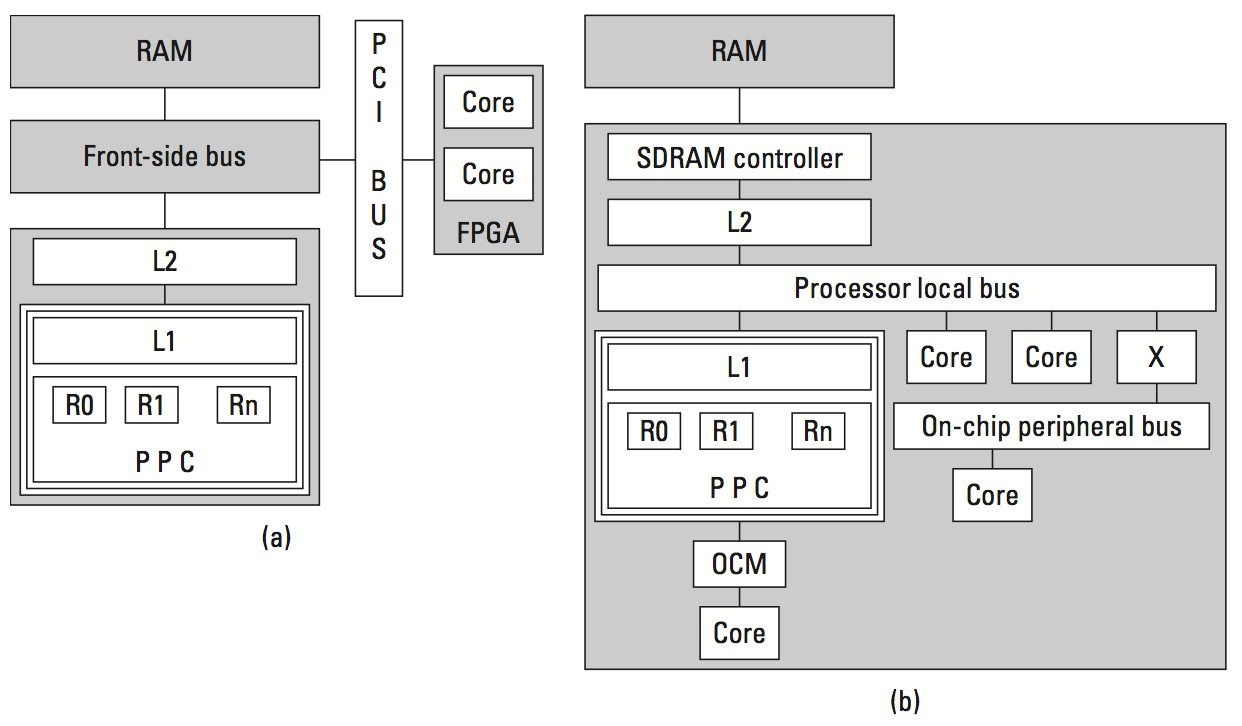
\includegraphics[width=1\textwidth]{img/f4-7.png}
			\caption{Situações na qual pode ocorrer bloqueio de estado. \textit{a)} Situação na qual existe um processador externo ao FPGA e sua memória interna é inacessível. \textit{b)} Situação onde o processador situa-se na plataforma FPGA. Fonte: \cite{Sass2010}.}
			\label{fig:4-7}
		\end{figure}

		Em ambos os casos mostrados na Figura \ref{fig:4-7} o FPGA (representado pelos \cores\ não possui autorização para o acesso aos registradores do processador (representados por $R_n$). Mesmo em \textit{b)} onde o processador é integrado à plataforma FPGA, não possui-se acesso sendo necessário a disponibilização manual deste.
	\end{description}


\subsection{Problema de Transferência de Estado}
	Estados afetados que estão presos necessitam de ser explicitamente comunicados e esta é feita por um processo chamado \textit{marshaling}.
    Assim, será feito um \textit{Marshaling} de grupos de elementos de um estado afetado de uma aplicação em registros lógicos que são explicitamente transferidos.

    Tendo a premissa que o processador possui o controle inicial, tem-se quatro tipos de registros que podem ser utilizados.
    Os dois primeiros, \textit{Type-I} e \textit{Type-F}, são utilizados para iniciar e outro para finalizar a transferência de um conjunto de elementos para o recurso, respectivamente.
    Os outros dois tipos de \textit{marshal} são usados repetidamente. Um quando o recurso é invocado (\textit{Type-CI}, do inglês \textit{copy-in}), e quando é completado (\textit{Type-CO}, do inglês \textit{copy-out}).
    %Um exemplo de \textit{Type-F} é quando tem-se um \core\ que acumula um valor em uma variável global. O registro \textit{Type-F} seria utilizado para ler o valor da variável após sua última invocação.

	Um processo de tradução pode ser incorporado com o \textit{marshaling}, sendo o exemplo a conversão de ponto flutuante para fixo quando transferido para um recurso o que acontece também com transformações mais complexas.
    %O agrupamento de elementos é lógico pelo fato do \textit{assembly} não significar estritamente que os elementos são copiados para uma memória de locação contínua.

	A forma mais simples de transferir estados é copiando os registros, parando o processador enquanto o recuso processa.
    Este é chamado de \textit{push} os dados no qual transmite o dado antes da transferência do controle. Ao final, realiza-se o \textit{pulls} dos dados.


    Embora simples uma transferência instantânea de estado não é sempre simples. Quando o estado afetado é grande mas o dado atua é pequeno, o padrão de acesso ao dado é randômico e a transferência lógica de registro é larga sendo mais vantajoso o uso de interfaces de comunicação para servir o recurso. Ou seja, utilizado quando o recurso foi designado para reduzir a latência da tarefa e a transferência do registo é pequena.
    Quando o registro lógico e o dado atual são largos, utiliza-se de padrão de acesso regula que transmite dados continuamente. É usado quando o recurso aumenta o \textit{throughput} e a redução de latência ou metas de performance não são possíveis.

    Isso é útil por exemplo na ordenação onde transferir um arranjo completo quando invocado é uma operação cara e desnecessária já que dependendo do algoritmo, pode-se utilizar apenas frações deste.

\end{comment}







\section{O Particionamento de \HS} \label{chap:desenvolvimento}

	%Para dar início ao problema, será considerado como aplicação um conjunto de instruções organizadas, como uma coleção de grafos de controle de fluxo especificando a sua ordem de execução.

	%Alguns fatores podem ajudar nas decisões de particionamento tal como expectativa de ganho de performance (Seção \ref{sec:performance}), os recursos utilizados em \hardware\ (Seção \ref{sec:recursos}), a forma na qual são usados e, talvez os mais importantes, quanto de sobrecarga de comunicação a decomposição impõe (Seção \ref{sec:comunicacao}) \todo{deixar?}e dificuldade de implementar um conjunto específico em \hardware\ (Seção \ref{sec:dificuldades}).

Algumas definições prévias:\todo[inline]{parei aqui}
	\begin{itemize}
    	\item \textbf{Recurso:} grupo conectado de instruções de uma aplicação de \design\ referencial de \software\ `adequado' para uma implementação em \hardware;

        O recurso pode variar de um pequeno conjunto de instruções até um modulo de \software\ completo consistente de múltiplas sub-rotinas. Como o tamanho dos recursos afetam na performance, a decisão de implementação em \hardware\ depende da sua melhoria no sistema por inteiro e mensura-se os recursos utilizados com relação a outros recursos candidatos.

        Se determinado que o recurso é vantagem, então os recursos de implementação em \hardware\ aumentam a arquitetura de \hardware.

        \item \textbf{Implementação em \hardware:} recurso adicional de uma específica aplicação;

        \item \textbf{Adequado:} descrevendo de forma mais geral no âmbito de sistemas embutidos, é a definição da situação na qual o projetista do sistema antecipa a percepção de vantagens na implementação em \hardware. %Para obter uma boa partição, geralmente deve-se examinar grupos que podem ser maiores ou menores que sub-rotinas definidas pelo programador.
    \end{itemize}

	\begin{figure}[!b] \centering
		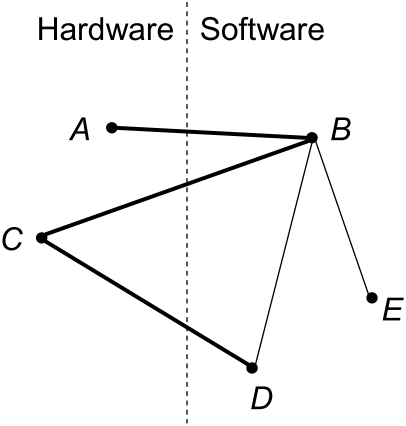
\includegraphics[width=0.18\textwidth]{img/partitioning.png}
		\caption{Representação Geral de um Particionamento em um grafo não direcionado. Os $\bullet$ (pontos) representam componentes da aplicação e as --- (linhas) seus respectivos fluxos de comunicação. A linha tracejada representa a divisão de níveis entre eles, sendo este \hs. Fonte: \cite{Mann2007}.}
		\label{fig:f4-4}
	\end{figure}

%\subsection{Declaração Formal do Problema}
%	Descreveremos problema segundo a definição de \cite{Arato2005, Mann2007} a seguir.

	%\subsection{Solução analítica para particionamento}
%\subsection{Visão Analítica Para o Particionamento}
\subsection{Declaração do Problema}
	Nesta seção será descrita as fórmulas matemáticas do problema de agrupamento de instruções em recursos e seus mapeamentos em \hardware\ ou \software.
	Segundo \cite{Sass2010}, a forma mais comum de transcrever é descrever manualmente o \core\ com um HDL utilizando \design\ referencial de \software\ como especificação, método utilizado para descrever o problema.

	No particionamento, muitos problemas práticos impactam diretamente na performance do sistema.
    Nem todos os problemas podem ser incorporados num modelo analítico \cite{Wang2016}, e por isso, só podemos esperar que as soluções matemáticas produzam uma uma resposta aproximada ao problema de particionamento ao utilizar a declaração formal.

	Muitas das entradas do modelo são estimadas ou aproximações no qual futuramente degrada a fidelidade de resultados.
    %Este é um fato relevante pois com isso, resolvendo o problema de particionamento `no papel', tem-se um particionamento que é próximo ao ótimo.
	%Assim, cabe ao \designer\ ser habilidoso em usar os guias e projetar uma solução mais refinada.
	Dessa forma, é mais eficiente usar uma combinação de técnicas \textit{ad hoc} e matemáticas para encontrar uma solução ótima ou aproximada do que simplesmente confiar numa intuição.


%\begin{comment}
%\subsection{Declaração do Problema}
	Já descrito as ferramentas matemáticas necessárias para descrever o problema fundamental do particionamento no Capítulo \ref{chap:revisao_bibliografica}, pode-se então, primeiramente, descrever formalmente o problema em termos de variáveis e descrever um algoritmo para encontrar uma solução aproximada.

		A ideia básica consiste em encontrar um particionamento para todos os blocos básicos de uma aplicação e então separá-los em \hs.
        Formalmente, procura-se por uma partição $ \mathcal{P} $ de todos os blocos básicos $ U $ de uma aplicação (Equação \ref{eq:bigcup})

        $$ U = \bigcup_{C \in \mathcal{C}} B(C) $$

		%$ C = (B,F) $
		Definida a partição e o universo, tem-se então um subconjunto $ \mathbb{C}\ |\ \mathbb{C} \subseteq U $, onde $ C \in \mathcal{C} $ é um vértice de um grafo de \design\ referencial de \software\ $ \mathcal{A} = (\mathcal{C}, \mathcal{L}) $ (oriundo da Equação \ref{eq:a}). O conjunto $ \mathbb{C} $, chamado conjunto de candidatos, contém todos os recursos arquiteturais potenciais, ou seja, o subconjunto de $ U $ que é esperado para melhorar a performance do sistema se implementado em um \hardware\ reconfigurável.
        Devido ao limite de recursos, deve-se refinar para o subconjunto $ \mathbb{D} \subseteq \mathbb{C} $ que maximiza nosso métrica de performance. Assim

		\begin{comment}
			\begin{eqnarray}
				\Gamma ( \mathbb{D}) \text{ é maximizado, e } \\
				\sum_{i \in \mathbb{d}} \vec{r}(i) < \vec{r}_{FPGA}
			\end{eqnarray}
		\end{comment}

		\begin{comment}
		\begin{table}[h]
			\begin{tabular}{rrcl}
			max                 & $\Gamma ( \mathbb{D})$               & ~   & ~                \\
			\textit{subject to} & $\sum_{i \in \mathbb{D}} \vec{r}(i)$ & $<$ & $\vec{r}_{FPGA}\label{eq:constraints}$
			\end{tabular}
		\end{table}
		\end{comment}

			\begin{equation}
					\begin{array}{rrcl}
					\text{max}                 & \Gamma ( \mathbb{D})               & ~   & ~                \\
					subject\ to & \sum_{i \in \mathbb{D}} \vec{r}(i) & < & \vec{r}_{FPGA}
					\end{array}
                    \label{eq:constraints}
			\end{equation}

		Algoritcamente, uma abordagem desse problema seria encontrar todas as partições de $ U $, sintetizando e \textit{profiling} cada partição, e então, quantitativamente avaliar cada $ \Gamma $. 
        %Como este é um problema linear inteiro (Seção \ref{sec:pli}) devido à alocação e utilização dos recurso físicos do FPGA, será escolhida uma abordagem heurística para tal \cite{Arato2003, Wang2016}.

\begin{comment}
\subsection{Abordagem Heurística}
	O problema de particionamento é essencialmente uma questão indireta de manipulação de parâmetros $ p(i) $ e $ \gamma(i) $ (tempo gasto em e ganho de performance, respectivamente) pelo rearranjo do particionamento $ \mathcal{X} $. Então seleciona-se os elementos de $ \mathcal{X} $ que satisfaz as restrições de recurso e maximiza a performance do sistema $ \Gamma $, Equação \ref{eq:constraints}.

	Uma metodologia heurística que pode ser aplicada informalmente é iniciar a partição natural provida pelo \design\ referencial de \software, ou seja, utiliza-se as sub-rotinas de uma aplicação original.

    Utilizando a ferramenta de \textit{profiling}, lista-se as sub-rotinas em ordem decrescente em tempo e verifica-se as que possuem maior valor $ p $. O valor de $ \gamma $ será estimado pela performance esperada a partir da implementação em \hardware\ e ao final, tem-se um ganho estimado do sistema para cada sub-rotina.

	Em seguida, quer-se manipular iterativamente a partição $ \mathcal{X} = \{ X_0, X_1, X_2, ...\} $ criando um novo subconjunto de blocos básicos por meio de operações de casamento e movimentações de blocos.
    A ideia em realizar alterações iterativas é encontrar mudanças que podem alterar os valores da fração $ p $ ou o valor de $ \gamma $.

    \begin{comment}
	\subsubsection{Fração do Tempo de Execução e Ganho de Performance} \label{sec:performance}
    \todo[inline]{Acho que esta parte do livro está errada}
		Uma forma de aumentar a fração de tempo gasta de uma sub-rotina, \todo{ou seja, diminuir seu tempo,} é torná-la maior na quantidade de recurso alocada a ela, por exemplo, casando vários blocos básicos num único bloco. Isso pode ser alcançado procurando por relações no grafo de chamadas ou, após a manipulação, por relacionamentos no grafo de controle de fluxo que conecta subconjuntos.

        Por exemplo, supondo que uma aplicação que teve seu tempo $ p(i) = 0,005 $ gaste:
        \begin{itemize}
        	\item $ 0,5\% $ numa sub-rotina \textit{A}; e
            \item $ 0,25\% $ nas sub-rotina \textit{B} e \textit{C}.
        \end{itemize}

        A fração de tempo gasto em \textit{A} pode ser duplicada pelo casamento de \textit{A, B} e \textit{C}. Entretanto, isso possui seu preço. Geralmente, aumenta-se o número de recursos utilizados e também pode aumentar no tamanho do subconjunto do sistema, decrescendo sua performance.
	\end{comme nt}

	\subsubsection{Ganho de Performance} \label{sec:performance}

		Para aumentar o ganho performance de recurso $ \gamma (i) $ necessita-se verificar o grafo de controle de fluxo do recurso e avaliar se uma mudança o tornará mais sequencial ou paralelo.

        Frequentemente, algoritmos que são inerentemente sequenciais, ou seja, uma forte dependência em seu fluxo ou dependências de controle, possuem melhor performance em processadores, por este não ter a sobrecarga de configurações de transistores e de possuírem melhor gerenciamento de energia nessas circunstâncias.
        Ou seja, simplesmente adicionar blocos básicos pode ter um efeito indesejável de aumentar o comportamento sequencial do recurso, reduzindo o valor de $ \gamma $.
        Entretanto, se um componente utilizar-se de menos recursos, então possui potencial de aumentar seu ganho de desempenho pela simplicidade. Exemplificando de uma forma mais geral, considara-se uma sub-rotina $ X $ e quebrando-a em duas sob-rotinas $ X – X' $ e $ X' $, onde a sub-rotina $ X – X' $ invoca $ X' $.
        Então se $ X' $ extrai partes de $ X $ que podem ser melhoradas em nível de \hardware\ deixando a parte sequencial em $ X – X' $, então $ \gamma $ de $ X' $ será maior que $ \gamma $ de $ X $ original e provavelmente necessitará de menos recursos.

        %Assim, supondo uma sub-rotina tome $ 93\% $ de tempo e provê um ganho de $ \gamma = 2 $, então a aplicação terá performance de $ \Gamma = 1.869 $. Entretanto, se uma parte da sub-rotina pode ser extraída aumentando o paralelismo, então é possível que a performance poderia aumentar em dez vezes tendo o $ \gamma = 20 $ e com isso, o tempo decrescendo para $ 83\% $. Esse particionamento gera um \speedup\ de $ \Gamma = 4.739 $.

		%A lei de Ahmdal tenta sempre aumentar a fração de tempo gasto na porção de código que acaba de ser melhorada.
        %No entanto, quando limitado os recursos, nem sempre é melhor.

		Com isso é importante notar que qualquer mudança no subconjunto pode afetar a performance para melhor ou pior.
        Em geral, heurísticas trabalham examinando os grafos da aplicação e então fazendo mudanças incrementais ao subconjunto de uma partição.
        Tais mudanças são guiadas pela tentativa de diminuir o tempo gasto em uma sub-rotina não aumentando dramaticamente seus recursos ou decrescendo sua performance; e a tentativa de aumentar a performance sem aumentar o tempo gasto em uma sub-rotina.


\begin{comment}
\subsection{\Benchmarks}
	\cite{Trindade2016}

	% intro
	Por serem um excelente mensurador de performance de aplicações e processadores, \designs\ têm feito de \benchmarks\ uma parte crítica do processo de \design\ de projetos.
	Uma vez que um \benchmark\ torna-se padrão e popular em um ramo de pesquisa, cria-se então uma alta pressão em aumento de performance por otimizações \cite{Hennessy2011}.

	% utilização de benchs no trabalho
	% arato2005
	Para a demonstração e validação da solução a ser desenvolvida, será utilizado %vários \benchmarks\ e exemplos randômicos largos.
	\benchmark\ de \textit{MiBench}.
	Esse \benchmark, segundo \cite{Guthaus2001} foi escolhido com base em um exame e comparação de um conjunto de aplicações embarcadas representativas comercialmente com o conjunto de \benchmarks\ SPEC2000 \cite{Case1995}.
\end{comment}
